\begin{figure}[htbp]
 \centering
 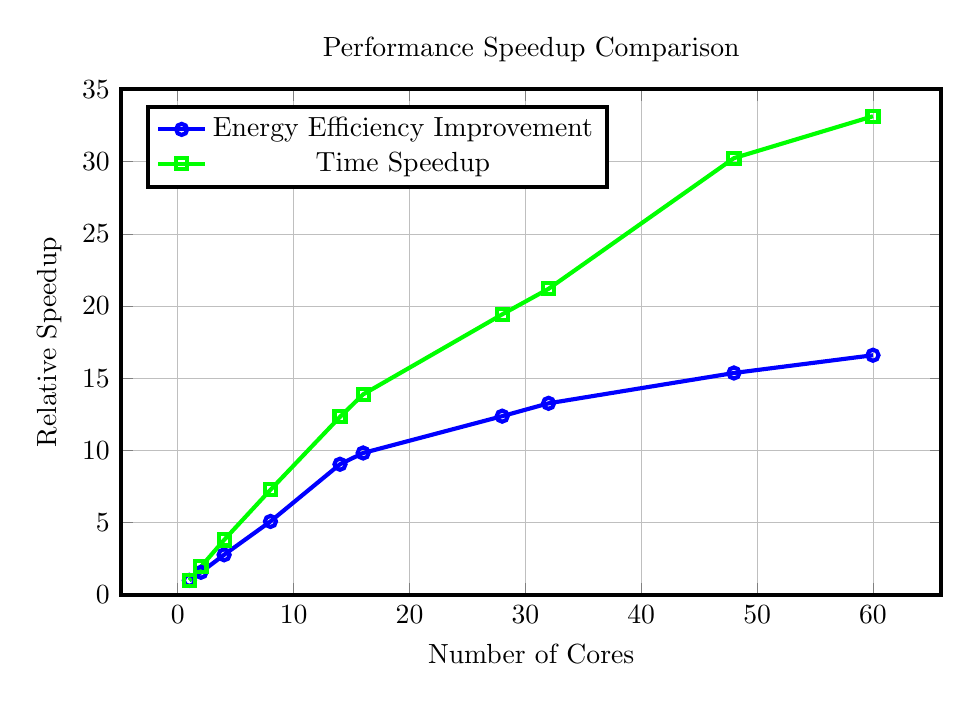
\begin{tikzpicture}
 \begin{axis}[
     xlabel={Number of Cores},
     ylabel={Relative Speedup},
     title={Performance Speedup Comparison},
     grid=both,
     grid style={line width=.1pt, draw=gray!10},
     major grid style={line width=.2pt,draw=gray!50},
     width=12cm,
     height=8cm,
     legend pos=north west,
     mark size=2pt,
     line width=1.5pt,
     ymin=0,
     ymax=35
 ]
 
 % Energy speedup (selected points for clarity)
 \addplot[color=blue, mark=o] coordinates {
     (1, 1)
     (2, 1.56)
     (4, 2.77)
     (8, 5.08)
     (14, 9.04)
     (16, 9.82)
     (28, 12.37)
     (32, 13.26)
     (48, 15.36)
     (60, 16.59)
 };
 
 % Time speedup (selected points for clarity)
 \addplot[color=green, mark=square] coordinates {
     (1, 1)
     (2, 1.94)
     (4, 3.8)
     (8, 7.27)
     (14, 12.32)
     (16, 13.88)
     (28, 19.42)
     (32, 21.19)
     (48, 30.24)
     (60, 33.14)
 };
 
 \legend{Energy Efficiency Improvement, Time Speedup}
\end{axis}
\end{tikzpicture}
\caption{Relative performance improvements showing time scales better than energy efficiency}
\label{fig:go-routines-speedup} 
\end{figure}


\begin{table}
  \centering
  \begin{tabular}{lcrcrc}
    \toprule
    Cores & Goroutines & Energy (J) & Relative Energy & Execution time (s) & Relative Time \\
    \midrule
    1             & 1          &  28,522.69         & ($1x$)              &  172.952          &  ($1x$)               \\
    1             & 2          &  28,919.31         & ($0.99x$)           &  175.381          &  ($0.99x$)            \\
    2             & 2          &  18,231.97         & ($1.56x$)           &   89.319          &  ($1.94x$)            \\
    2             & 4          &  18,224.50         & ($1.57x$)           &   89.275          &  ($1.94x$)            \\
    4             & 4          &  10,304.27         & ($2.77x$)           &   45.508          &  ($3.8x$)             \\
    4             & 8          &  10,299.06         & ($2.77x$)           &   45.482          &  ($3.8x$)             \\
    8             & 8          &  \textbf{5,617.27} & (\textbf{$5.08x$})  &   \textbf{23.781} &  (\textbf{$7.27x$})   \\
    8             & 16         &  5,580.52          & ($5.11x$)           &   23.594          &  ($7.33x$)            \\
    14            & 14         &  3,155.30          & ($9.04x$)           &   14.034          &  ($12.32x$)           \\
    14            & 28         &  3,151.93          & ($9.05x$)           &   14.001          &  ($12.35x$)           \\
    16            & 16         &  2,904.52          & ($9.82x$)           &   12.456          &  ($13.88x$)           \\
    16            & 32         &  3,018.54          & ($9.45x$)           &   12.435          &  ($13.91x$)           \\
    28            & 28         &  2,306.35          & ($12.37x$)          &    8.906          &  ($19.42x$)           \\
    28 \textbf{*} & 28         &  \textbf{2,271.71} & (\textbf{$12.56x$}) &    \textbf{7.613} &  (\textbf{$22.72x$})  \\
    28            & 56         &  2,314.29          & ($12.32x$)          &    7.791          &  ($22.2x$)            \\
    28 \textbf{*} & 56         &  \textbf{2,290.85} & (\textbf{$12.45x$}) &    \textbf{8.815} &  (\textbf{$19.62x$})  \\
    32            & 32         &  2,151.74          & ($13.26x$)          &    8.163          &  ($21.19x$)           \\
    32 \textbf{*} & 32         &  \textbf{2,109.37} & (\textbf{$13.52x$}) &    \textbf{6.822} &  (\textbf{$25.35x$})  \\
    32            & 64         &  2,121.88          & ($13.44x$)          &    8.101          &  ($21.35x$)           \\
    32 \textbf{*} & 64         &  \textbf{2,142.21} & (\textbf{$13.31x$}) &    \textbf{6.896} &  (\textbf{$25.08x$})  \\
    48            & 48         &  1,856.93          & ($15.36x$)          &    5.718          &  ($30.24x$)           \\
    48            & 96         &  1,848.47          & ($15.43x$)          &    5.673          &  ($30.48x$)           \\
    60            & 60         &  1,744.76          & ($16.35x$)          &    5.357          &  ($32.28x$)           \\
    60            & 120        &  1,737.80          & ($16.41x$)          &    5.320          &  ($32.5x$)            \\
    60            & 200        &  1,724.73          & ($16.54x$)          &    5.255          &  ($32.91x$)           \\
    60            & 250        &  1,719.49          & ($16.59x$)          &    5.218          &  ($33.14x$)           \\
    \bottomrule
  \end{tabular}
  \caption[Go goroutines and threads]{Go goroutines and threads used in the tests, where \textbf{*} means the execution has been fixed to a single CPU}
  \label{tab:go-routines-cores}
\end{table}
